\documentclass[onecolumn, oneside, a4paper, 11pt]{memoir}

\usepackage[utf8]{inputenc}
\usepackage[T1]{fontenc}

% Paths
\newcommand{\figs}{../figs}
\newcommand{\data}{../data}

% Fonts
\usepackage{newpxtext,newpxmath}
\renewcommand*\sfdefault{cmss}

% References
\usepackage{hyperref}

% Units
\usepackage[detect-weight=true, binary-units=true]{siunitx}
\DeclareSIUnit\flop{Flops}

% Math
\let\openbox\undefined
\usepackage{amsthm}
\usepackage{amsmath}
\usepackage{amssymb}
\usepackage{bm}

\theoremstyle{remark}
\newtheorem{ex}{Exercise}
\newtheorem*{sol}{Solution}

% Graphics
\usepackage{graphicx}
\usepackage{caption}
\usepackage{subcaption}
\graphicspath{{../figs/}}

% Tikz
\usepackage{tikz}
\usetikzlibrary{positioning,shapes,arrows,calc,intersections}
\usepackage{pgfplots}
\usepgfplotslibrary{dateplot}
\pgfplotsset{compat=1.8}

% Colors
\definecolor{darkblue}{HTML}{00688B}
\definecolor{darkgreen}{HTML}{6E8B3D}
\definecolor{cadet}{HTML}{DAE1FF}
\definecolor{salmon}{HTML}{FFB08A}

% Listings
\usepackage{textcomp}
\usepackage{listings}
\lstset{
  keywordstyle=\bfseries\color{orange},
  stringstyle=\color{darkblue!80},
  commentstyle=\color{darkblue!80},
  showstringspaces=false,
  basicstyle=\ttfamily,
  upquote=true,
}
\lstdefinestyle{fortran}{
  language=Fortran,
  morekeywords={for},
  deletekeywords={status},
}
\lstdefinestyle{c}{
  language=C,
  morekeywords={include},
}
\lstdefinestyle{shell}{
  language=bash,
}

\begin{document}

\pagestyle{empty}

\begin{center}
  {\Huge \bfseries \scshape
    Introduction to \\[0.2\baselineskip] Supercomputing} \\[2\baselineskip]
  {\Large TMA4280 $\cdot$ Problem set 6} \\[2\baselineskip]
\end{center}

\textbf{Note that}
\begin{itemize}
\item this problem set is mandatory;
\item you can work on it in groups with \emph{up to} 3 members;
\item you should write a report describing your solution (max 12 pages);
\item you should write your \emph{names} on the report (no student numbers);
\item the source code should be handed in together with the report (and not as
  part of it);
\item please make sure that you have answered all the questions;
\item the due date is Friday, April 15, 2015;
\item the report will count 30\% towards the final grade.
\end{itemize}

\setsecnumdepth{none}
\maxsecnumdepth{none}

\section{Problem description}

Consider the solution of the two-dimensional Poisson problem,
\begin{align*}
  -\nabla^2 u &= f & \text{ in } \Omega = (0,1) \times (0,1), \\
  u &= 0 & \text{ on } \partial\Omega.
\end{align*}
Here, $f$ is a given right hand side and $u$ is the solution.

Assume that we discretize this problem on a regular finite difference grid with
$(n+1)$ points in each spatial direction. Hence, the grid size is $h=1/n$. We
use the standard 5-point stencil to discretize the Laplace opkerator.

In order to solve the system of algebraic equations, we apply the
diagonalization methods discussed in class. In particular, we apply the Discrete
Sine Transform (DST) in order to obtain a solution of this problem in
$\mathcal{O}(n^2\log n)$ floating point operations.

\begin{ex}
  Write a program to solve the Poisson problem with $P$ processes using the
  algorithms described above. You can choose $f \equiv 1$ for the initial
  development.

  Use the provided routines to compute the DST and its inverse based on the FFT.
  See Appendix A for details on compiling, linking and running the serial
  version of the Poisson solver. Use the MPI communication library to develop
  your program for a distributed memory parallel computer, and OpenMP to use $t$
  threads on each MPI process. See Appendix C for comments on the transpose
  operation.
\end{ex}

\begin{ex}
  Run your parallel program on \emph{Vilje}. Obtain detailed timing results for
  different combinations of $n=2^k$ and $P, t$. In particular, demonstrate that
  your program functions correctly for selected values of $P$ in the range
  $1 \leq P \leq 36$. Follow the procedure described in Appendix B.

  \textbf{Note:} Having a program that runs quickly is useless unless the answer
  is correct.

  \textbf{Note:} It is sufficient and strongly recommended that you test the
  correctness of your program on a small problem size before solving larger
  problems.
\end{ex}

\begin{ex}
  Run your program with $n=16384$ and $pt=36$, i.e. with about $270$ million
  grid points on 36 threads/processes. Does the hybrid model work better, worse
  or equivalent to the pure distributed memory model? Explain your observations.
\end{ex}

\begin{ex}
  Report the speedup $S_p$ as well as the parallel efficiency $\eta_p$ for
  different values of $n$ and $p$. Th parallel efficiency is defined as
  $\eta_p = S_p / p$.

  How do your timing result scale with the problem size $n^2$ for a fixed number
  of processors? Is it as expected? Do you see an improved speedup if you
  increase the problem size?

  \textbf{Note:} To obtain consistent and reliable timing results, submit
  individual runs as different jobs.
\end{ex}

\begin{ex}
  Modify the given $f$ to be a function of your own choice. As an example, you
  could choose $f$ to be a smooth function like
  \[
    f(x, y) = \text{e}^x \sin(2\pi x) \sin(2 \pi y).
  \]
  Another example is to let $f$ represent point sources, e.g. $f \equiv 0$ in
  the whole domain except at two chosen gridpoints where $f=-1$ and $f=1$
  respectively.

  Run your program with the new right hand side $f$ for a particular $n$ and
  $p$. Do you have to modify anything related to the parallel implementation
  when you change $f$, i.e. when solving a different Poisson problem?
\end{ex}

\begin{ex}
  Discuss how you would modify the numerical algorithm to deal with the case
  where $u \not= 0$ on $\partial\Omega$, i.e. for non-homogeneous Dirichlet
  boundary conditions. You do not have to implement this.
\end{ex}

\begin{ex}
  In the exercise and lectures we have assumed that the domain is the unit
  square, i.e. $\Omega = (0,1) \times (0,1)$. Discuss how you would modify the
  Poisson solver based on diagonalization techniques if the domain instead is a
  rectangle with sides $L_x$ and $L_y$. You can still assume a regular finite
  difference grid with $n+1$ points in each spatial direction. Does this
  extension of the original method change anything in terms of your parallel
  implementation? You do not have to implement this.
\end{ex}

\section{General comments}

It will be emphasized that the program is well parallelized and load balanced.
It will also be important that the program is well organized and easy to
understand. It is allowed to use more memory than the minimum required if it
speeds up the program, but do so with care.

A report describing the results of parallelization of a scientific problem
typically contains
\begin{itemize}
\item a description of the problem;
\item a discussion of possible solution strategies;
\item a brief explanation of the finished program;
\item a description of the computer on which the numerical results were
  obtained, which compiler (with version) and compiler options you used and
  other relevant information, such as libraries used and their versions;
\item numerical results (preferably plots)
\item analysis (theoretical and experimental) of the performance of the
  algorithm and its implementation (time usage, speedup and efficiency as
  functions of problem size and number of processes or threads);
\item a discussion of bottlenecks and possible improvements; and
\item possibly a listing of relevant parts of the source code.
\end{itemize}

\section{A \quad Compiling and linking}

The serial code ships with a CMake build system. You can generate a build system
using
\begin{lstlisting}
module load intelcomp
module load cmake
CC=icc FC=ifort cmake . -DCMAKE_BUILD_TYPE=Release
\end{lstlisting}
assuming you are located in the folder with the \texttt{CMakeLists.txt}. On
success this will generate a makefile, and you can then build and run the
program using
\begin{lstlisting}
make
./poisson 128
\end{lstlisting}
The first statement builds the program, while the second runs it on a single
processor with $n=128$. Note that $n$ must be a power of two.

By default CMake does not show you the compiler commands. You can see them by doing
\begin{lstlisting}
make VERBOSE=1
\end{lstlisting}

It is recommended to perform out-of-tree builds. For example, using a
\texttt{build} folder:
\begin{lstlisting}
mkdir build
cd build
cmake ..
\end{lstlisting}

The CMake setup has options for compiling with MPI and OpenMP. They are on by
default, but can be disabled at the configuration stage:
\begin{lstlisting}
cmake . -DENABLE_OPENMP=0 -DENABLE_MPI=0
\end{lstlisting}

\section{B \quad Verification of correctness}

One way to verify that the code works correctly is to do a \emph{convergence
  test}. Following this approach, we first assume an exact solution to our
Poisson problem. For example, we can assume that the exact solution is given as
\[
  u(x,y) = \sin(\pi x) \sin(2\pi y).
\]
This solution satisfies the boundary conditions.

Next, evaluate $-\nabla^2 u$, which should be equal to $f$, i.e.
\[
  f(x,y) = -\nabla^2 u = 5\pi^2 \sin(\pi x) \sin(2\pi y).
\]
Assuming the given data $f$ we now solve the Poisson problem numerically, and
compare the computed solution with the exact solution at the grid points. The
maximum pointwise error should decrease to zero as $\mathcal{O}(h^2)$the given
data $f$ we now solve the Poisson problem numerically, and compare the computed
solution with the exact solution at the grid points. The maximum pointwise error
should decrease to zero as $\mathcal{O}(h^2)$. Remember that finding the maximum
pointwise error will require communication.

\section{C \quad Comments on the transpose operation}

The implementation of the transpose operation is trivial in a serial context. In
a parallel context, using a distributed memory programming model, it is quite
tricky. In this case the transpose of a matrix will involve all-to-all
communication.

Part of the solution of this exercise requires a parallel implementation of the
transpose operation. We are given a matrix of a certain dimension. We can
distribute the matrix so that each process is responsible for a certain number
of columns (or rows).

The most convenient way to implement the transpose operation is to use the MPI
function \texttt{MPI\_Alltoallv}. For a detailed description of this function,
please use Google.

\begin{figure}[htbp]
  \begin{center}
    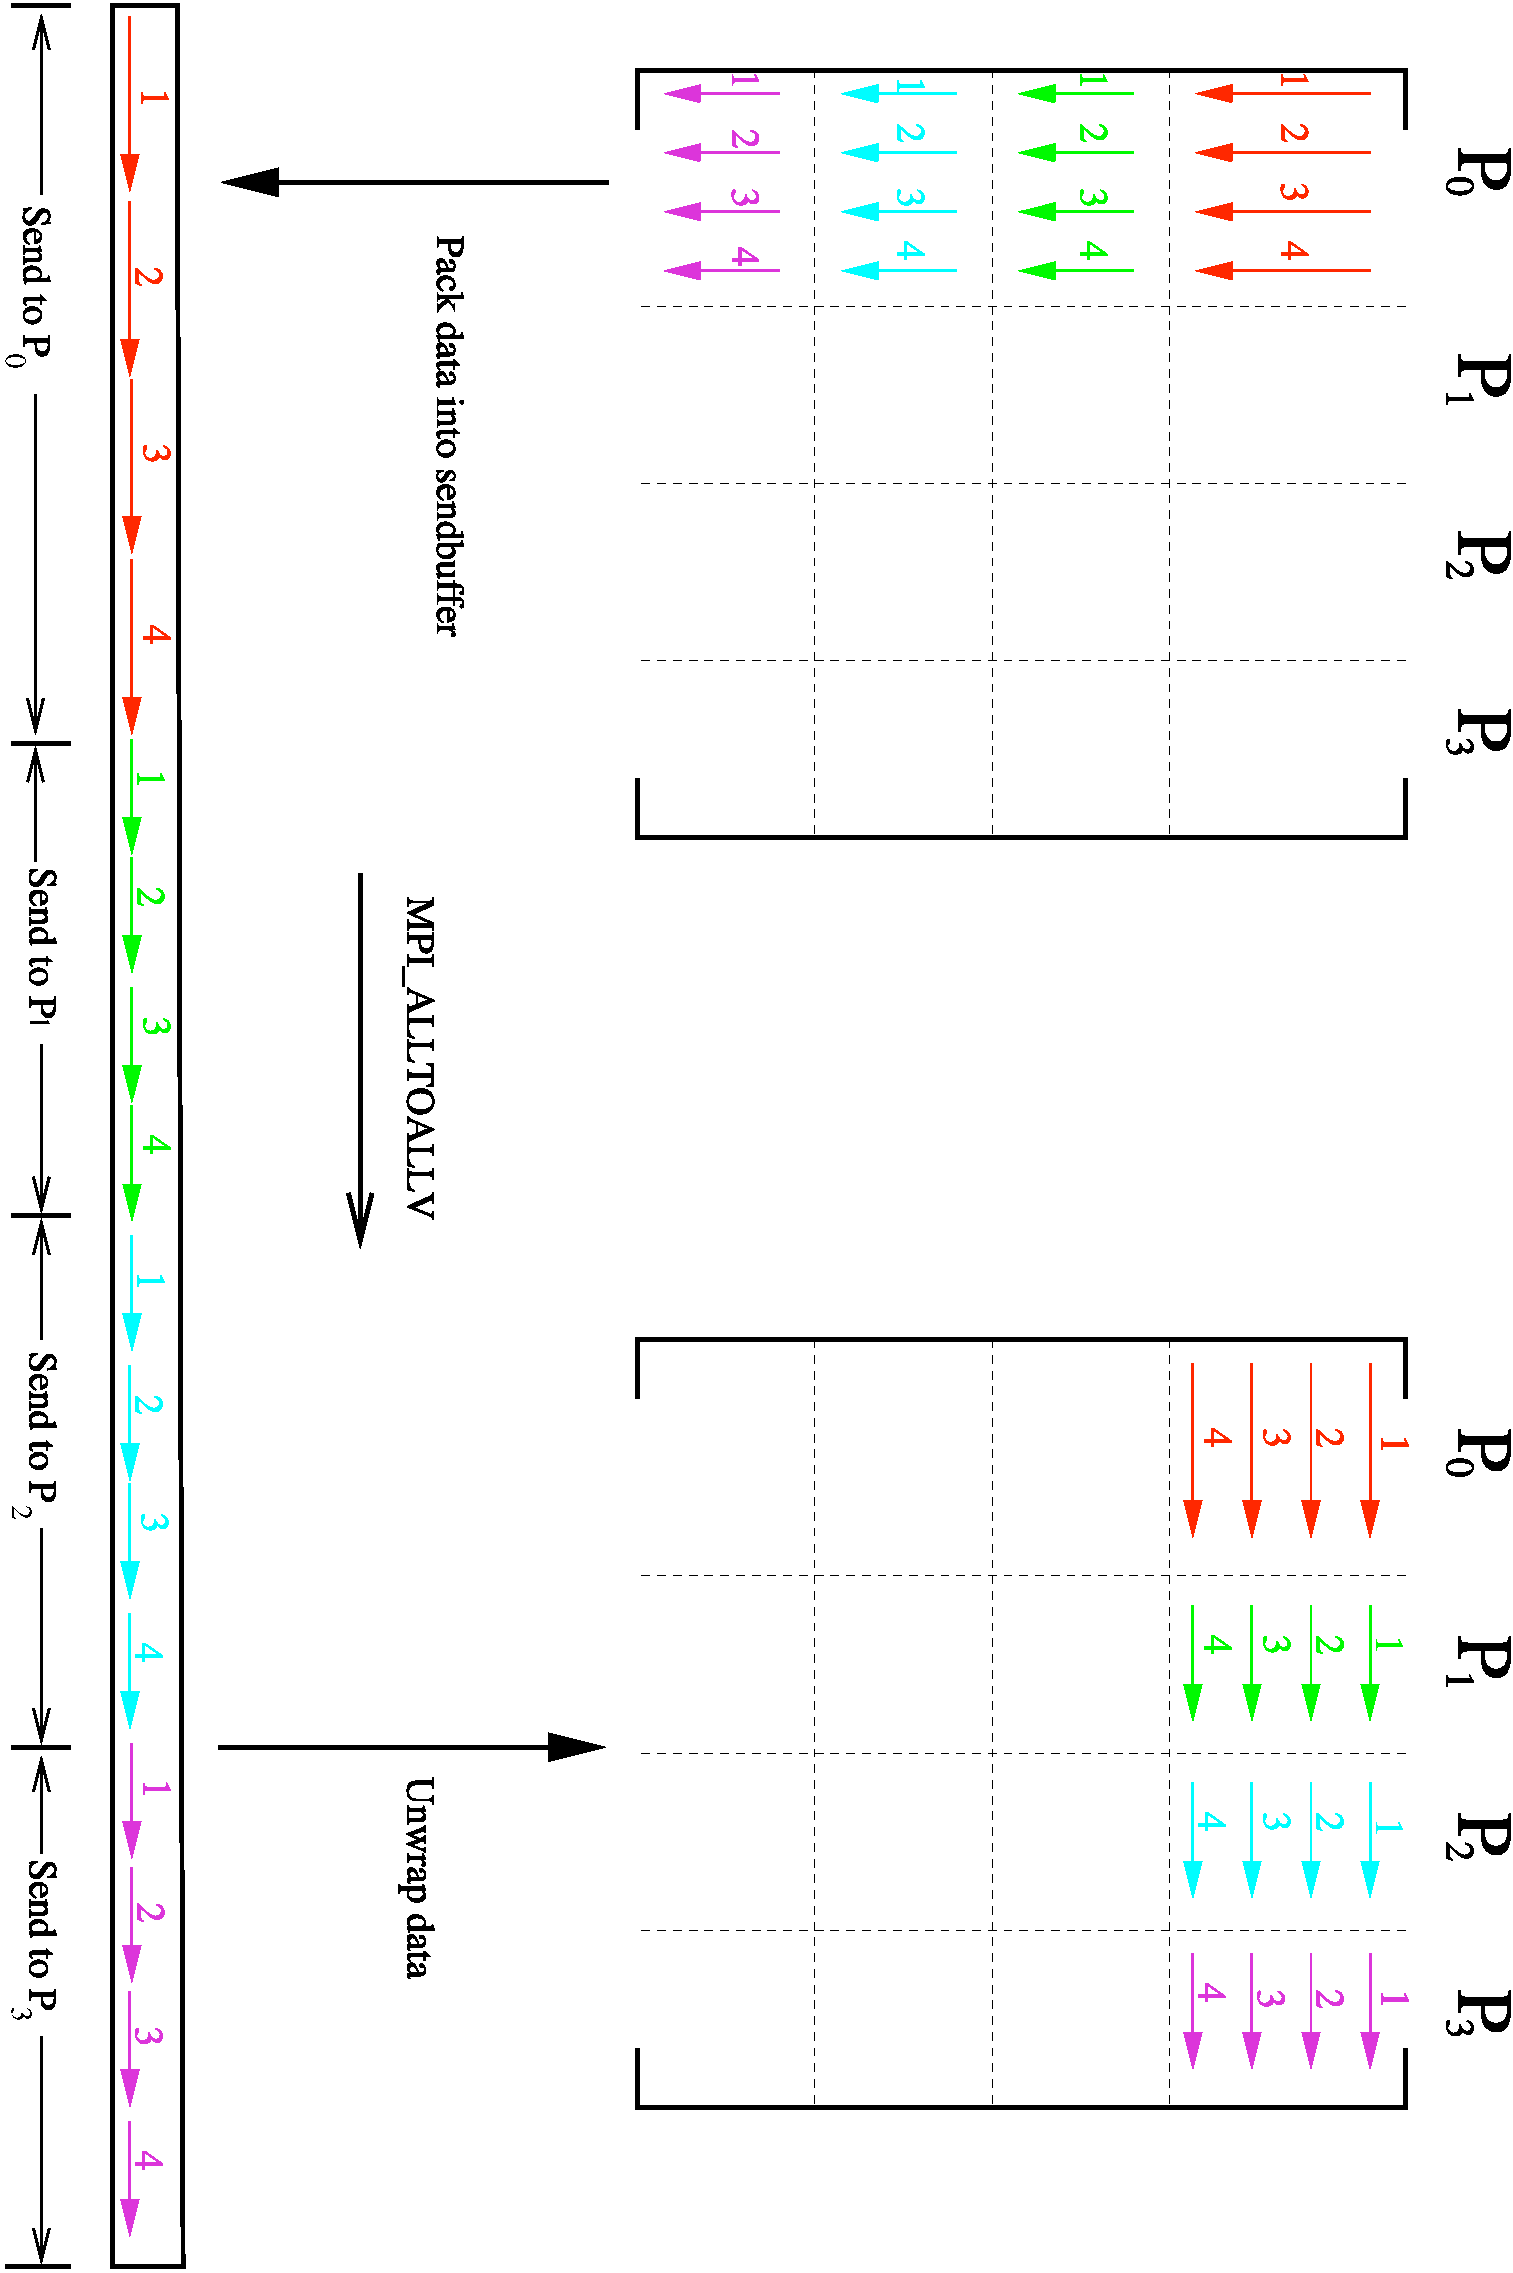
\includegraphics[scale=0.4]{\figs/matrix_blocktranspose}
  \end{center}
  \caption{
    The transpose operation using message passing:
    the packing and unpacking of data.
    The figure is due to Bjarte H{\ae}gland.
  }
  \label{}
\end{figure}

\end{document}
